

\section{1. Visualisation 3D: contexte, orientation}


\subsection{Contexte}


\begin{frame}[t]
\frametitle{1. Visualisation 3D: contexte}
\vspace{-0.3cm}
\begin{block}{Premier \textit{DGtal meeting} (4 janvier 2011)}
\begin{itemize}
\item Outils de visualisation pour les primitives 2D.
\item M�canisme simple permettant de montrer des r�sultats li�s � diff�rents modules:  
\begin{itemize}
\item Topologie (Jacques-Olivier lachaud)
\item G�om�trie (David Coeurjolly, Tristan Roussillon)
\item Domaine (Guillaume Damian)
\end{itemize}
\end{itemize}
\end{block}

\visible<2>{\rput(6,-1.7){
\begin{minipage}{\textwidth}
\begin{center}
\begin{tabular}{ccc}
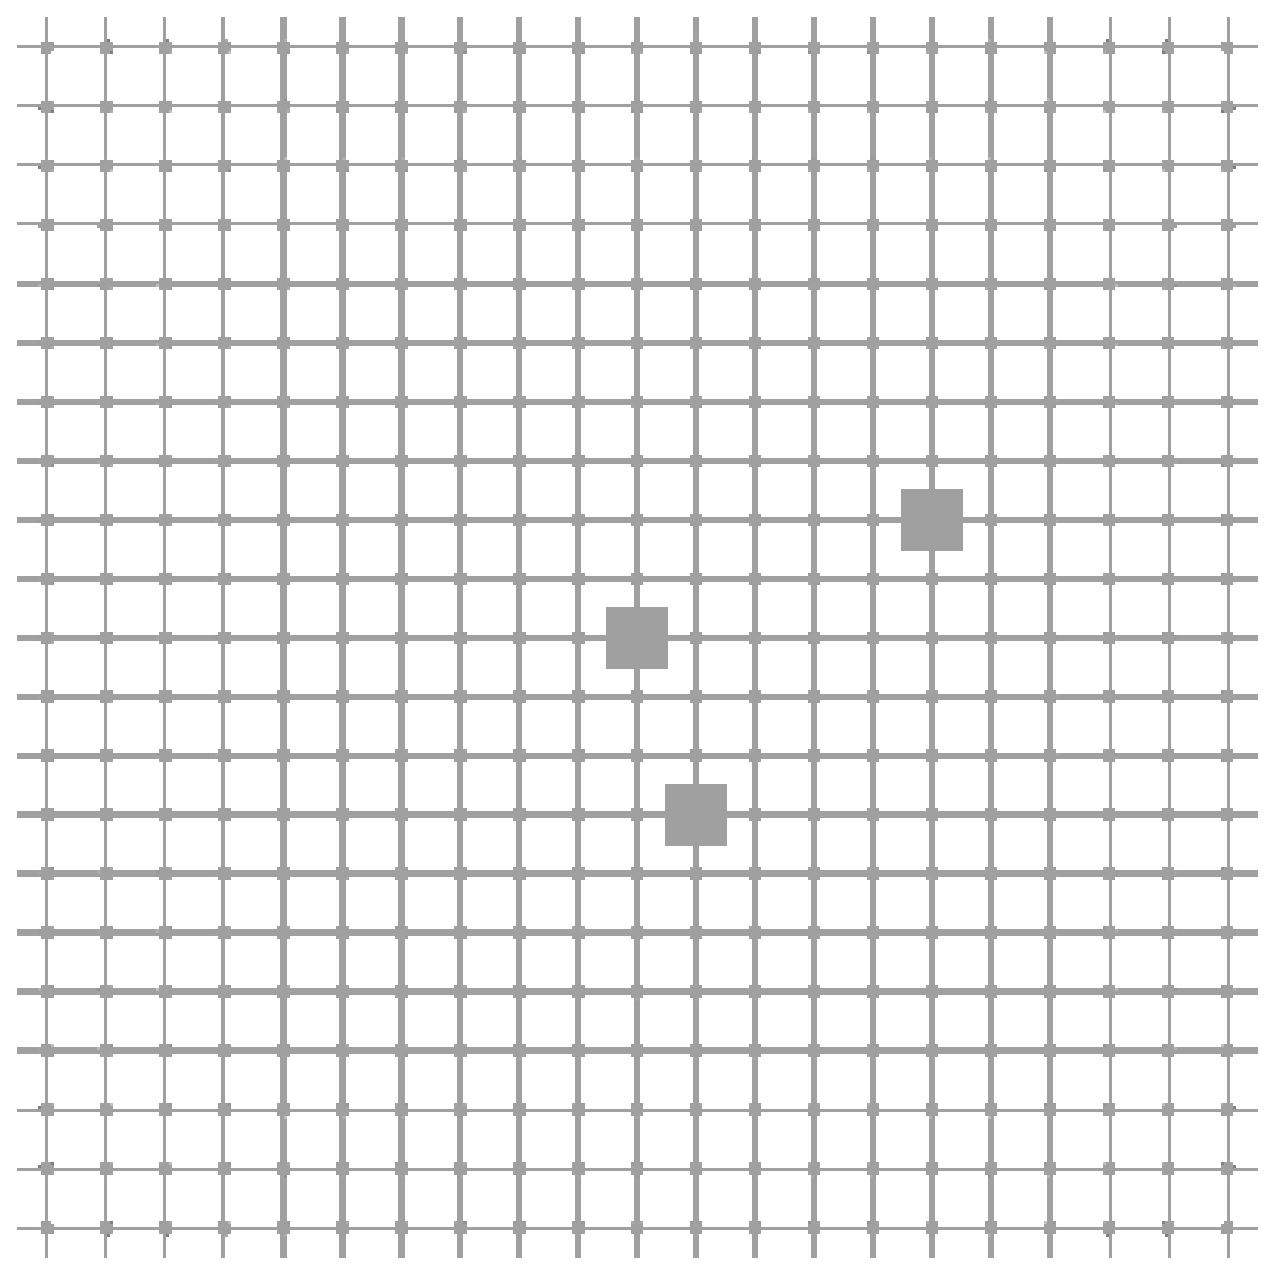
\includegraphics[height=0.15\textwidth]{Images/gallerie1.eps}&
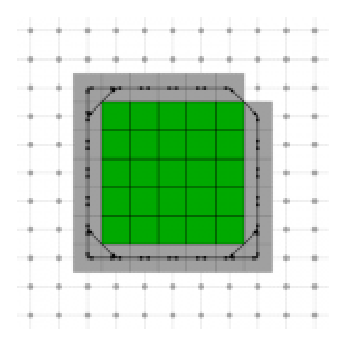
\includegraphics[height=0.15\textwidth]{Images/gallerie2.eps}&
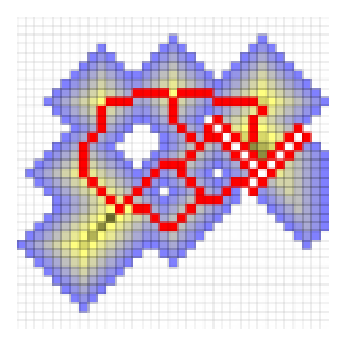
\includegraphics[height=0.15\textwidth]{Images/gallerie3.eps}\\
$\vcenter{ \hbox{
\includegraphics[height=0.15\textwidth]{Images/gallerie4.eps}}}$ &
$\vcenter{ \hbox{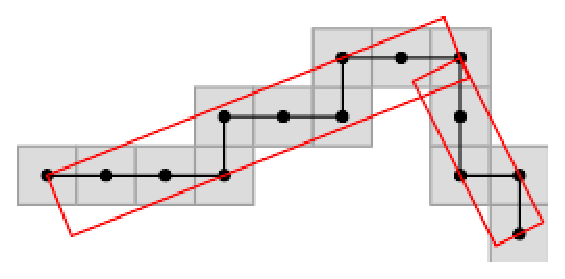
\includegraphics[height=0.1\textwidth]{Images/gallerie5.eps}}}$ &
$\vcenter{ \hbox{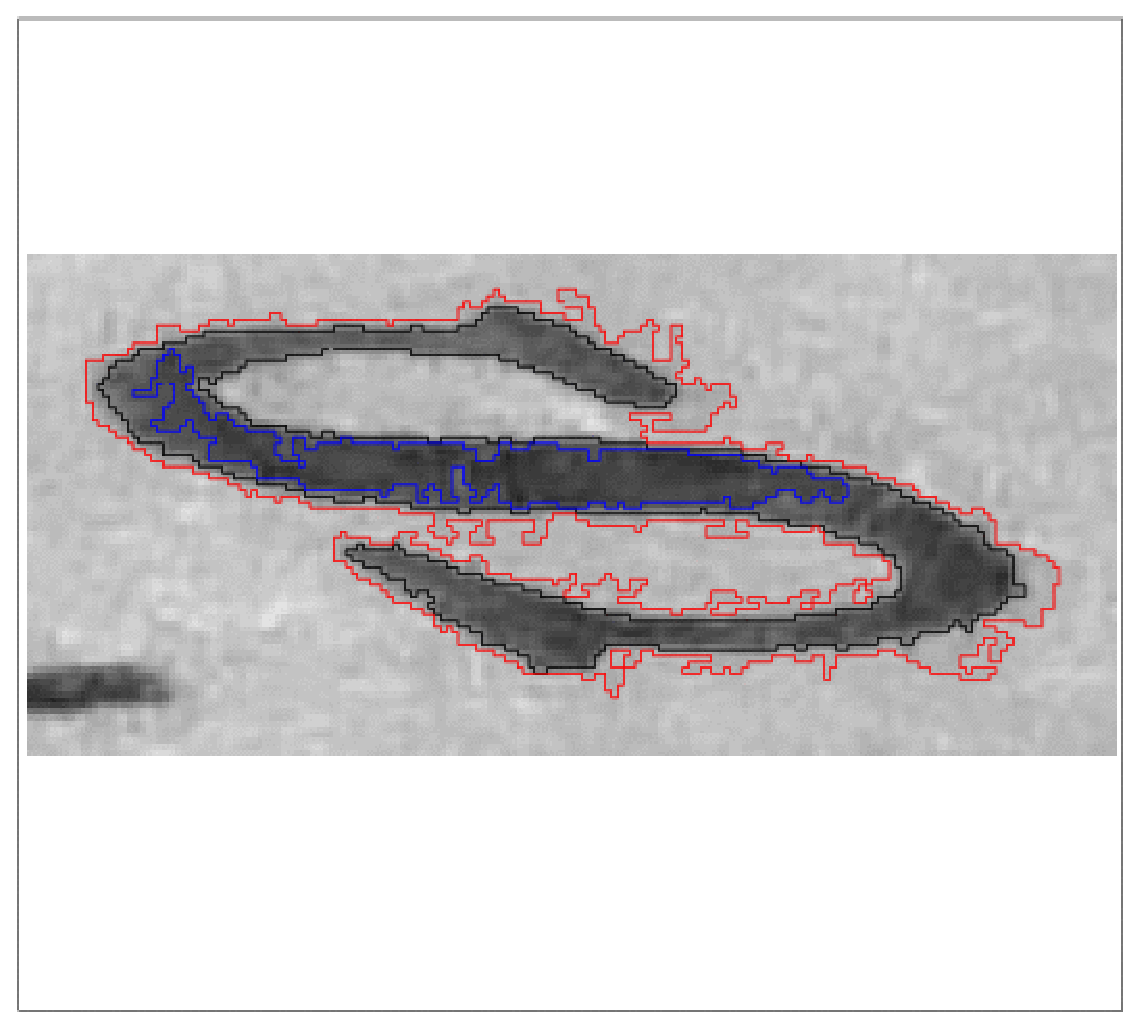
\includegraphics[height=0.15\textwidth]{Images/gallerie6.eps}}}$ \\
\end{tabular}
\end{center}
\end{minipage}}}
\vspace{-0.3cm}

\visible<3->{
\begin{block}{Objectifs pour la visualisation  3D}
\begin{itemize}
\item Garder un syst�me simple par flux (m�me primitive).
\item Manipulation, �dition d'objet 3D. 
\item Plusieurs directions: 
\begin{itemize}
\item Bertrand Kerautret: visualisation bas�e \textit{OpenGL, LibQGLviewer}
\item Jacques-Olivier Lachaud: visualisation bas�e \textit{Open Inventor SoQT}
\item Martial Tola: visualisation (2D/3D) bas�e sur \textit{CAIRO \footnote{Biblioth�que de rendu vectoriel: \url{http://cairographics.org}}}  


\end{itemize}
\end{itemize}

\end{block}
}
\end{frame}









\subsection{Orientation}


\begin{frame}[t]

\frametitle{1. Visualisation 3D: objectif}

{\large{Inspir� du m�canisme de \texttt{Board2D} (initialement bas� sur \texttt{LibBoard}\footnote{(Copyleft, LGPL) 2007 S�bastien Fourey - GREYC ENSICAEN}) }}

\begin{block}{}
\begin{itemize}
\item Chaque primitive capable de s'auto dessiner. 
\item V�rifier le concept \texttt{CDrawableWithBoard2D} (concept v�rifi� avec \textit{\textcolor<3>{red}{boost}}).  
\item<4-> M�canisme de ``flux'' avec l'op�rateur \texttt{< \hspace{-0.2cm}<}.
\item<6-> Exportation en diff�rents formats (pdf, eps, fig, gif, png). 
\end{itemize}
\end{block}


\visible<2,3>{%
\begin{footnotesize}
\begin{itemize}
\item \texttt{std::string styleName() const}
\item \texttt{DrawableWithBoard2D* defaultStyle(const std::string \& mode = "" ) const}
\item \texttt{void selfDraw( Board2D \& ) const}
\item<3> \texttt{\color{red}{BOOST\_CONCEPT\_ASSERT((CDrawableWithBoard2D<TDrawableWithBoard2D>));}}
\end{itemize}
\end{footnotesize}

}

\visible<5->{%
\visible<6,7>{\rput(3;6){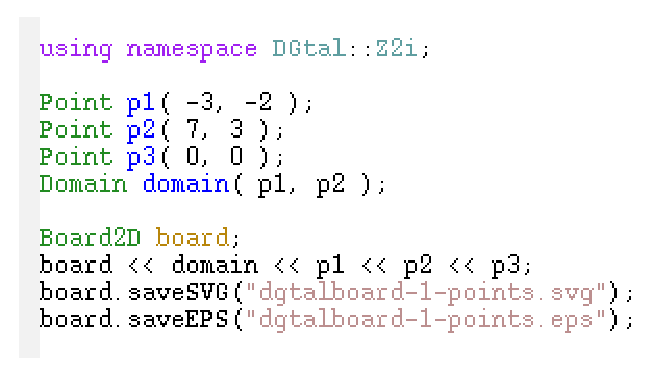
\includegraphics[width=6cm]{Images/codeExBoard2D.eps}}}%
\visible<7>{\rput(9;4){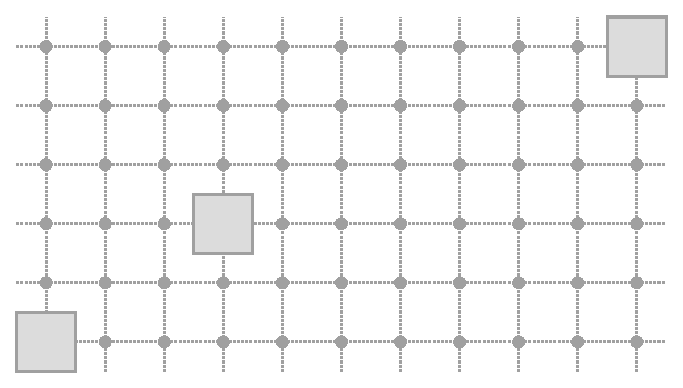
\includegraphics[width=5cm]{Images/dgtalboard-1-points.eps}}}%
\visible<5>{\rput(3;9){
\begin{minipage}{0.5\textwidth}
\begin{itemize}
\item[] \texttt{\footnotesize{Board2D board;}} 
\item[] \texttt{\footnotesize{board \texttt{< \hspace{-0.2cm}<} object;}} 
\end{itemize}%
\end{minipage}}}
}%

\end{frame}


